% \documentclass[notes=only]{beamer}
\documentclass{beamer} 

% Deutsch
\usepackage[german]{babel} % deutsch und deutsche Rechtschreibung
\usepackage[utf8]{inputenc} % Unicode Text 
\usepackage[T1]{fontenc} % Umlaute und deutsches Trennen
\usepackage{textcomp} % Euro
% \usepackage[hyphens]{url}
\usepackage{emptypage} % Wirklich leer bei leeren Seiten
\usepackage{listings}
\usepackage{xcolor}

\definecolor{codegreen}{rgb}{0,0.6,0}
\definecolor{codegray}{rgb}{0.5,0.5,0.5}
\definecolor{codepurple}{rgb}{0.58,0,0.82}
\definecolor{backcolour}{rgb}{0.95,0.95,0.92}

\lstdefinestyle{mystyle}{
    backgroundcolor=\color{backcolour},   
    commentstyle=\color{codegreen},
    keywordstyle=\color{magenta},
    numberstyle=\tiny\color{codegray},
    stringstyle=\color{codepurple},
    basicstyle=\ttfamily\footnotesize,
    breakatwhitespace=false,         
    breaklines=true,                 
    captionpos=b,                    
    keepspaces=true,                 
    numbers=left,                    
    numbersep=5pt,                  
    showspaces=false,                
    showstringspaces=false,
    showtabs=false,                  
    tabsize=2
}
\lstset{style=mystyle}



\usepackage[yyyymmdd]{datetime}
\renewcommand{\dateseparator}{--}
%Information to be included in the title page:
\title{Smartbit}
\author{Marius Cerwenetz}
\institute{Institut für Softwaretechnik und Datenkommunikation}
\date{\today}

\beamertemplatenavigationsymbolsempty



\begin{document}

\frame{\titlepage}
\addtobeamertemplate{navigation symbols}{}{%
    \usebeamerfont{footline}%
    \usebeamercolor[fg]{footline}%
    \hspace{1em}%
    \insertframenumber/\inserttotalframenumber
}
\begin{frame}
\frametitle{Agenda}
% \tableofcontents[pausesections]
\tableofcontents

\end{frame}

\section{Einführung}
\begin{frame}
    \frametitle{Schwierigkeiten beim Programmierenlernen}
    \begin{itemize}
        \item Programmier-Neulinge
        \item Grundkonzepte
        \item Theoretische Übungsaufgaben
    \end{itemize}
\end{frame}

\begin{frame}
    \frametitle{Microcontroller als Alternative}
    \begin{itemize}
        \item Interaktive Aufgaben
        \item Ausgabemöglichkeiten (LEDs, Piepser, Aktoren)
        \item Ausprobieren
    \end{itemize}
\end{frame}



\begin{frame}
    \frametitle{Vorteile Smartphones gegenüber Microcontroller-Schaltungen}
    \begin{itemize}
        \item Hohe Verfügbarkeit
        \item Keine Verdrahtungsfehler
        \item Unabhängige Spannungsversorgung
        \item Zahlreiche Sensoren bereits integriert
        \item Drahtlose Verbindungstechnologien (WLAN, Bluetooth, UMTS/LTE)
        \item Zweckgebundene Ausgabemöglichkeiten
    \end{itemize}
\end{frame}

\begin{frame}
    \frametitle{Smartbit}
    \begin{alertblock}{Probleme}
        \begin{itemize}
            \item Anbindung in Programmierumgebungen
            \item Smartphone-App
        \end{itemize}
    \end{alertblock}
    \begin{block}{Lösung}
        Lösung zur Kommunikation mit dem Smartphone
    \end{block}
\end{frame}

\section{Anforderungen}
\begin{frame}
    \frametitle{Anforderungen}
    \begin{itemize}
        \item UI-Elemente als Ausgabe
        \item Sensordatenübermittlung
        \item Geringe Latenzen
        \item Sicherheit
    \end{itemize}
\end{frame}
\note{Everything you want}

\section{Smartbit}
\begin{frame}
    \frametitle{Aufbau der Smartbit-Lösung}
    \begin{columns}
        \begin{column}{0.3\textwidth}
            \centering
            
\includegraphics[width=5em]{images/lib.pdf}
            Bibliothek
        \end{column}
        \begin{column}{0.3\textwidth}
            \centering
            
\includegraphics[width=5em]{images/server.pdf}
            Middleware
        \end{column}
        \begin{column}{0.3\textwidth}
            \centering
            
\includegraphics[width=5em]{images/android.pdf}
            Android-App
        \end{column}
    \end{columns}
\end{frame}

\begin{frame}[fragile]
    \frametitle{Schnittstelle zum Programmcode}
    Funktionsaufrufe für Sensorwerte und Ausgaben.
    \begin{columns}
        \begin{column}{0.3\textwidth}
            Einbindbar in:
            \begin{itemize}
                \item C
                \item Java
                \item Python
            \end{itemize}
        \end{column}
        \begin{column}{0.6\textwidth}
            \begin{lstlisting}[language=python]
from  smartbit import Phone
p = Phone()
accel = p.get_x_accelo()
p.write_text("hallo")
            \end{lstlisting}
        \end{column}

    \end{columns}
    
   
\end{frame}

\begin{frame}
    \frametitle{Smartphone-App}
    \centering
    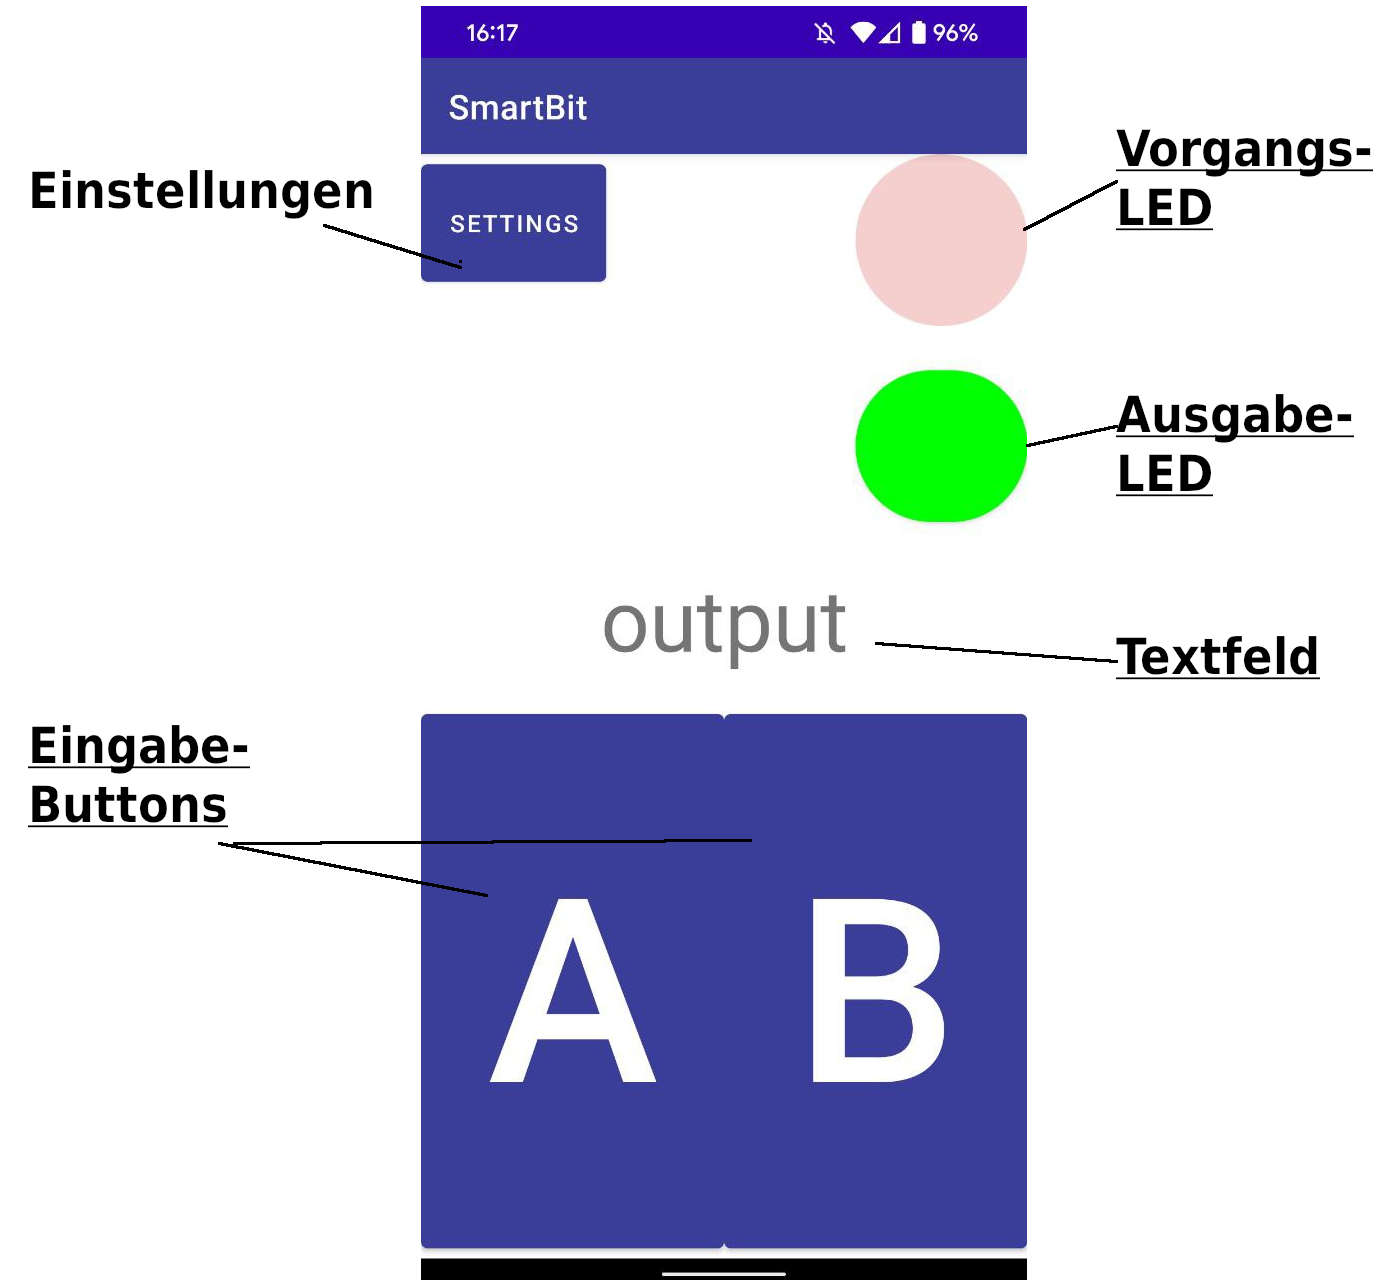
\includegraphics[height=0.9\textheight]{images/app_initial.png}
\end{frame}

\begin{frame}[fragile]
    \frametitle{Middleware}
    \begin{center}
    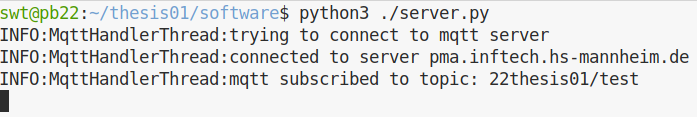
\includegraphics[width=0.8\textwidth]{images/middleware.png}
    \end{center}
\end{frame}

\section{Architektur}
\begin{frame}
\end{frame}
\subsection*{Übersicht der Gesamtarchitektur}
\subsection*{Nachrichtenformate}
\subsection*{Funktionsweise der Bibliotheken}
\subsection*{Funktionsweise der Middleware}
\subsection*{Funktionsweise der Smartphone-App}

\section{Evaluation}
\begin{frame}
\end{frame}
\section{Fazit und Ausblick}
\begin{frame}
\end{frame}





\end{document}